\documentclass[border = 10pt,tikz]{standalone}
\usetikzlibrary{chains}
\usetikzlibrary{positioning}
\begin{document}

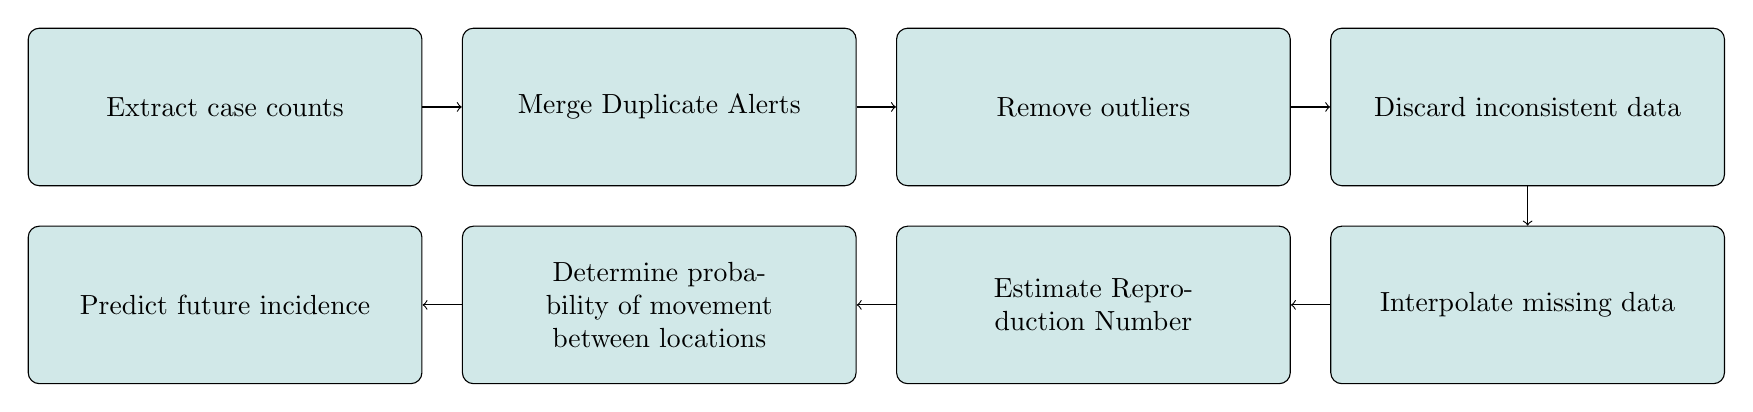
\begin{tikzpicture}[start chain=1 going right,
                    start chain=2 going left,
                    node distance=5mm,
                    every join/.style=->,
                    every node/.style={draw,
                      rectangle,
                      rounded corners,
                      minimum width = 5cm,
                      minimum height = 2cm,
                      text width = 4cm,
                      text=black,
                      text opacity=1,
                      align=center,
                    fill=teal!60}]
 \pgfsetfillopacity{0.3}
\node (a) [on chain=1,join] {Extract case counts};
\node (b) [on chain=1,join] {Merge Duplicate Alerts};
\node (c) [on chain=1,join] {Remove outliers};
\node (d) [on chain=1,join] {Discard inconsistent data};
\node (e) [on chain=2, below = of d,join] {Interpolate missing data};
\node (f) [on chain=2,join] {Estimate Reproduction Number};
\node (g) [on chain=2,join] {Determine probability of movement between
  locations};
\node (h) [on chain=2,join] {Predict future incidence};
\draw[->] (d) -- (e);
\end{tikzpicture}
\end{document}


